\documentclass[12pt]{article}
\usepackage{../../template}
\title{Lecture 7}
\author{niceguy}
\begin{document}
\maketitle

\section{Negative Bias}

Recall that if a negative voltage is applied to a diode, there is a $V_{ZK}$ before which leakage current is negligible and is approximately constant. There is an avalanche past that point with slope $\frac{1}{r_z}$, where $r_z$ is a small value. We can consider this as a linearised circuit, where there is a voltage source in the opposite direction to current (internal voltage), and a resistor with resistance $r_z$.

\section{Zener Diode as Shunt Regulator}

A shunt regulator keeps voltage constant. We can use a doide as a shunt regulator by attaching it parallel to a desired voltage. This is because if the desired voltage overcomes $V_{ZK}$, it will essentially be a conductor with an internal voltage. Once that voltage is overcome, all the "excess" current is drawn into the diode, so voltage output is regulated.

\begin{figure}[h]
    \begin{center}
    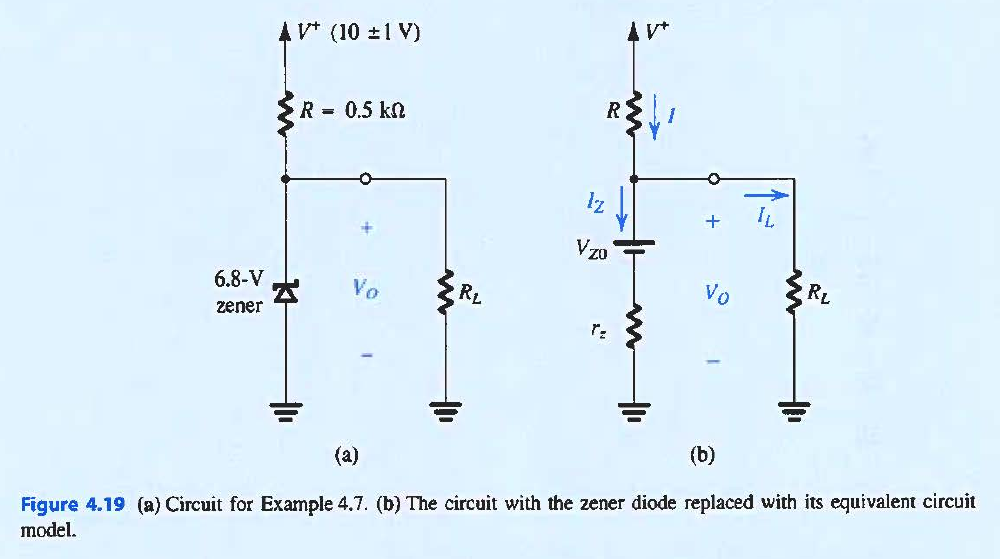
\includegraphics[width=\textwidth]{shunt.png}
    \end{center}
\end{figure}
    

\end{document}
